\documentclass[main.tex]{subfiles} 
\begin{document}

\section*{Metode \& Gjennomføring}
\label{sec:2}

Pedagogikkforsker Nordahl skriver at utfordringen er ikke at skolen mangler data, men at data ofte i lite grad blir
systematisk analysert og senere aktivt brukt for å forbedre praksisen (\citeNP[s. 9, i Forord]{hell07}).
I denne oppgaven er dataen innsamling av elevbesvarelser og mine egne skriftlige tilbakemeldinger.
Jeg har valgt å fremheve noen av disse skriftlige tilbakemeldinger for å analysere min egen praksis.
Dataen er også ment til å brukes i læringsrettet kontekst, der elevene kan få individuelle 
tilbakemeldinger og fremovermeldinger. 

Videre har jeg også valgt å benytte meg av kvalitativ forskningsmetode. Ved kvalitative metoder 
får en ofte anledning til å gå mere i dybden på materialet og man kommer tett på subjektene, men derfor er metoden også 
mere ressurskrevende og man må derfor begrense antall forsøksobjekter. Forskerne kaller det å "mette" materialet, noe som 
vil si flere intervjuer neppe vil avdekke noe avgjørende nytt (\citeNP{hoff13}). Jeg har hatt personlige samtaler med 10 
av 20 elever som tok kartleggingstesten. Elevene hadde ulike resultater og derfor også ulike former for tilbakemeldinger 
og fremovermeldinger.

Jeg valgte å fokusere på elevenes kunnskap rundt følgende kompetansemål \newline
(\citeNP{udirLP}) :
\begin{itemize}
\item finne og diskutere sannsyn gjennom eksperimentering, simulering og berekning i daglegdagse samanhengar og spel
\item beskrive utfallsrom og uttrykkje sannsyn som brøk, prosent og desimaltal
\end{itemize}
Ved design av kartleggingsprøven i sannsynlighet, ble disse kompetansemålene brukt som veiledning til utformingen av 
kartleggingsprøven.

\subsection*{Kartleggingsprøven i sannsynlighetsregning}

Før kartleggingsprøven ble brukt, jobbet elevene en uke med sannsynlighetsregning. Med mine observasjoner fra denne uken 
og kompetansemålene, utformet jeg testen sammen med en annen praksisstudent. Hensikten med kartleggingsprøven 
var å få oversikt over elevers ferdigheter i sannsynlighetsregning og hjelpe de med å avdekke deres
svakheter og misoppfattelser.

\citeA{skov98} kartlegger type oppgaver etter det han kaller 
\mbox{\emph{opgaveparadigmet} :}
%\footnote[2]{\citeA{skov98} beskriver oppgaveparadigmet som et læringsmiljø der læreren 
%innleder med å gjennomgå nytt stoff, deretter gjennomgås utvalgte oppgaver, hvor elever regner oppgaver, enten 
%individuelt eller i grupper. \emph{En matematikkundervisning, der er strukturert efter opgaveparadigme, føjer seg ind i 
%\guillemotleft oppgavediskursen\guillemotright} (\citeNP[s. 28]{skov98}).} 
klassiske lukkede oppgaver og åpne oppgaver 
vs. \emph{undersøgelseslandskaber} eller utforskende oppgaver. 
%I tabellen tallfester han disse oppgavetypene etter i hvilken grad de er tilnærmet virkeligheten. 
Videre klassifiserer \citeA[s. 215]{olma15} type oppgaver fra rike og åpne oppgaver 
til lukkede oppgaver. Jeg kommer derimot ikke til å bruke tabellen (\citeNP[s. 28]{skov98})) og klassifiseringen til 
\citeA[s. 215]{olma15} når jeg drøfter oppgavene fra kartleggingsprøven. Jeg vil begrense meg til elevenesbesvarelser 
og heller fokusere på hvordan jeg kan bruke kartleggingsprøver i vurderingsarbeidet til å fremme læring.

%\begin{figure}[h!]
%\centering
%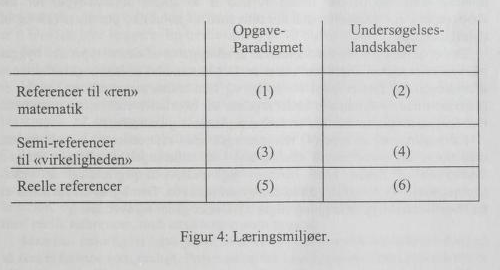
\includegraphics[scale = 0.7]{../figures/laeringsmiljoer.png}
%\caption{Kilde: \protect\citeA{skov98}.}
%\label{fig:skov98}
%\end{figure}

\end{document}
